\documentclass[article,A4,12pt]{llncs}

% Conditional compilation.
% NOTE: If you set fullversionfalse, just compile ONCE so that TOC stays unchanged.
\newif\iffullversion
\fullversiontrue
%\fullversionfalse

\usepackage[T1]{fontenc}
\usepackage{amsmath}
\usepackage{amssymb}
\usepackage{amsfonts}
\usepackage{mathrsfs, bm}

\usepackage{graphicx}
\usepackage{tabularx}
\usepackage{subfig}
\usepackage{epsf,times}
\usepackage{color}
\usepackage{wrapfig}
\usepackage{cases}
\usepackage{multicol}

\usepackage[T1]{fontenc}
%\newcommand{\tmname}[1]{\textsc{#1}}
%\newcommand{\tmop}[1]{\ensuremath{\operatorname{#1}}}
%\newcommand{\tmsamp}[1]{\textsf{#1}}
%\newcommand{\tmtextsc}[1]{{\scshape{#1}}}
%\newcommand{\tmtextsl}[1]{{\slshape{#1}}}
%\newcommand{\tmtexttt}[1]{{\ttfamily{#1}}}

\leftmargin=0.0cm
\oddsidemargin=0.5cm
\evensidemargin=0.5cm
\topmargin=0cm
\textwidth=16.0cm
%\textheight=21.5cm
\textheight=20.0cm
\pagestyle{plain}
\setlength{\columnsep}{20pt}

\def\m{\mathbf{m}}
\def\H{\mathbf{H}}
\def\E{\mathbf{E}}
\newcommand{\vepsi}{{\varepsilon}}
\def\hnorm#1#2{\vert\,#1\,\vert_{#2}}
\newcommand{\R}{{\mathbb R}}
\newcommand{\Sph}{{\mathbb S}}
\def\x{\mathbf{x}}
\def\hvec{\overline{\mathbf{h}}}
\def\evec{\overline{\mathbf{e}}}

\newcommand{ \etal}{\mbox{\emph{et al. }}}

\newcommand\vect[1]{\mbf{#1}}
\newcommand{\mbf}[1]{\mbox{\boldmath$#1$}} 
\newcommand{\RC}[1]{#1 $\times$ #1 $\times$ #1}
\def\um{$\mu$m}
\def\C{$^{\circ}\mathrm{C}$}

\newcommand{\Rmnum}[1]{\expandafter\@slowromancap\romannumeral #1@}

% DEFINITION OF CUSTOM FONT SIZE
\newcommand{\customfontA}{\fontsize{50}{55}\selectfont}
\newcommand{\customfontB}{\fontsize{14.4}{20}\selectfont}
\newcommand{\customfontC}{\fontsize{30}{35}\selectfont}

\DeclareMathAlphabet{\mathpzc}{OT1}{pzc}{m}{it}

\def\clovek#1{\noindent\bgroup\vbox{\noindent#1}\egroup\vskip1em}



\begin{document}



%%%%%%%%%%%%%%%%%%%%%%%%%%%%%%%%%%%%%%%%%%%%%%%%%%%%%%%%%%%%%%%%%%%%%%%%%

\pagestyle{empty}

\vbox{}
\begin{figure}[!ht]
%\hspace{-4mm}

\includegraphics[width=8cm]{imgp/logo.png}
\vspace{18mm}
\end{figure}
\vbox{}
\vspace{0.5cm}


\begin{figure}[!ht]
\begin{center}
\vspace{-6mm}
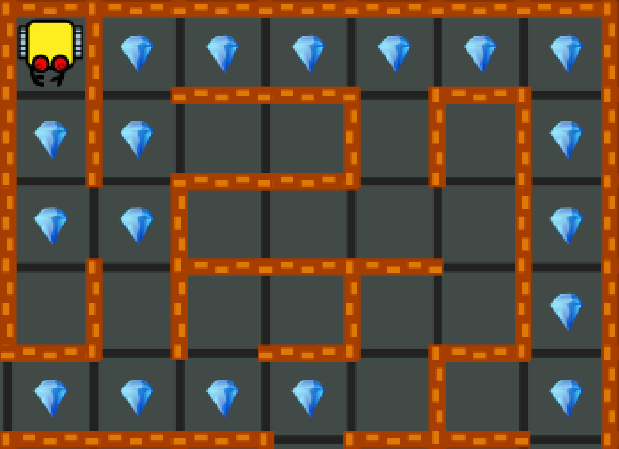
\includegraphics[width=0.26\textheight]{imgk/karel-logo.png}\ \ \ \ \ \ 

\includegraphics[width=0.2\textheight]{imgp/python-logo.png}
\vbox{}
\vspace{-9mm}
\end{center}
\end{figure}
\begin{center}
\vspace{2.8cm}
{\huge \bf Solution Manual}
\end{center}
\vbox{}
\begin{center}
\iffullversion
\else
\vspace{2mm}
\centerline{\huge \color{red}{PREVIEW}}
\fi
\vfill
{\large
{\bf Pavel Solin}, University of Nevada, Reno\\
{\bf Salih Dede}, Coral Academy of Science, Reno
}
\end{center}
\newpage
\vbox{}
\vfill
\begin{center}
{\large
This solution manual is part of the online course 
{\em Intro to Programming with Karel the Robot and Python} 
({\tt http://introtoprogramming.net}) and its use is allowed 
with current subscription only. Distribution or sharing is not allowed. \\
}
\vfill

Copyright 2012 FEMhub Inc. All rights reserved.
\end{center}




\section*{}
\small

\normalsize

\newpage
%{\ }
\setcounter{tocdepth}{2}
\tableofcontents
%\pagestyle{plain}

\newpage

\pagestyle{plain}
\setcounter{page}{1}

%%%%%%%%%%%%%%%%%%%%%%%%%%%%%%%%%%%%%%%%%%%%%%%%%%%%%%%%%%%%%%%%%%%%%%%%%

\part{Karel the Robot}

\section{Introduction}

\subsection{Review questions}

\begin{enumerate}
\item Name the university where Karel the Robot was created.
  \begin{itemize}
    \item A4: Stanford
  \end{itemize}
\item What is the programming language that you should learn after Karel?
  \begin{itemize}
    \item A2: Python
  \end{itemize}
\item What is the biggest conceptual difference between Karel and standard
      procedural programming languages such as Python, C, C++ or Fortran?
  \begin{itemize}
    \item A3: Karel does not know math.
  \end{itemize}
\item Where does Karel live and what objects does he like to collect?
  \begin{itemize}
    \item A1: Karel lives in a maze and he likes to collect gems.
  \end{itemize}
\item What is the command that moves the robot one step forward?
  \begin{itemize}
    \item A3: go
  \end{itemize}
\item What is the command that turns the robot to the left?
  \begin{itemize}
    \item A4: left
  \end{itemize}
\item What is the command that turns the robot to the right?
  \begin{itemize}
    \item A2: right
  \end{itemize}
\item What is the command to pick up a gem from the ground?
  \begin{itemize}
    \item A3: get
  \end{itemize}
\item What is the command to drop a gem on the ground?
  \begin{itemize}
    \item A1: put
  \end{itemize}
\item What sensor helps the robot avoid crashing into walls?
  \begin{itemize}
    \item A2: wall
  \end{itemize}
\item What sensor helps the robot detect gems?
  \begin{itemize}
    \item A3: gem
  \end{itemize}
\item What sensor does the robot use to check whether he has any gems in his bag?
  \begin{itemize}
    \item A4: empty
  \end{itemize}
\item What sensor helps the robot detect his orientation?
  \begin{itemize}
    \item A2: north
  \end{itemize}
\item What sensor helps the robot detect whether he is at home?
  \begin{itemize}
    \item A3: home
  \end{itemize}
\item What is the most important skill in computer programming?
  \begin{itemize}
    \item A2: Designing great algorithms.
  \end{itemize}
\end{enumerate}

\section{Launching Karel}

\subsection{Review questions}

\begin{enumerate}
\item What can you do with displayed Karel projects that you clone into your account?.
  \begin{itemize}
    \item A4: View, run, edit, save, whatever, they are all yours!
  \end{itemize}
\item What are the four modes of the Karel application?
  \begin{itemize}
    \item A1: Manual mode, Build mode, Program mode, Game mode.
  \end{itemize}
\item What is the difference between Levels 1 and 2?
  \begin{itemize}
    \item A4: In Level 2 programs can contain conditions, loops, and custom commands.
  \end{itemize}
\end{enumerate}

\section{Section A - Operating the Robot in Manual Mode}

\subsection{Review questions}

\begin{enumerate}
\item How can Karel be switched to Manual mode?
  \begin{itemize}
    \item A3: By pressing the Manual mode button.
  \end{itemize}
\item Look at  the arrows and decide which direction the robot is facing!
  \begin{itemize}
    \item A2: South
  \end{itemize}
\item What is the function of the following button?
  \begin{itemize}
    \item A4: Turn left.
  \end{itemize}
\item Select one or more correct statements from the four options below!
  \begin{itemize}
    \item A3: The last button on the right will turn the robot to the left.
  \end{itemize}
\item After you press the following button, the robot will:
  \begin{itemize}
    \item A2: Turn right and face West.
  \end{itemize}
\end{enumerate}

\section{Section B - Bridge to Programming}

\subsection{Review questions}

\begin{enumerate}
\item Where do we enter programs for Karel?
  \begin{itemize}
    \item A4: In input cells.
  \end{itemize}
\item Do we have to write one command per line?
  \begin{itemize}
    \item A3: No, but it makes the code easier to read.
  \end{itemize}
\item The robot's initial situation is as shown in the image. His bag with gems is empty. 
\begin{figure}[!ht]
\begin{center}
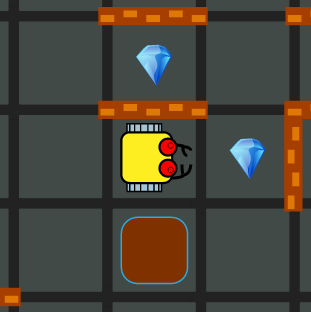
\includegraphics[width=4cm]{imgk/maze-0.png}
\end{center}
\end{figure}
\noindent
      Read the following program and select one or more correct statements!
\begin{verbatim}
go
right
get
go
right 
go
\end{verbatim}
  \begin{itemize}
    \item A2: The robot will return home with one gem in the bag.
  \end{itemize}
\item The robot's initial situation is the same as in the previous question. He has no gems 
in his bag. Read the following program and select one or more correct statements from the four options below!
\begin{verbatim}
go
get
left
go
left
go
get
right
right
go
right
go
put
go
left 
go
\end{verbatim}
  \begin{itemize}
    \item A4: The robot will not return home and he will have only one gem in the bag.
  \end{itemize}
\end{enumerate}

\subsection{Programming exercises}

\subsubsection*{B01 - Go Command}
\begin{verbatim}
go
go
\end{verbatim}

\subsubsection{B02 - Get Command}
\begin{verbatim}
go
get
go
get
go
get 
go
\end{verbatim}

\subsubsection{B03 - Left and Right Commands}
\begin{verbatim}
left
go
left
go
get
right
go
left
go
\end{verbatim}

\subsubsection{B04 - Put Command}
\begin{verbatim}
go
get
left
left
go
go
put
left
left
go
left 
go
\end{verbatim}

\section{Intermission - Algorithms, Programs, and Bugs}

\subsection{Review questions}

\begin{enumerate}
\item What is an {\em algorithm}?
  \begin{itemize}
    \item A4: Sequence of logical steps leading to the solution of the given task.
  \end{itemize}
\item What is a {\em program}?
  \begin{itemize}
    \item A3: Algorithm that is translated from human language to programming language.
  \end{itemize}
\item If the robot does something unexpected, what is the most probable reason for that?
  \begin{itemize}
    \item A4: Our algorithm contains a logical mistake.
  \end{itemize}
\item What of the following is a {\em logical} mistake?
  \begin{itemize}
    \item A1: Mistake in an algorithm that causes the robot to do something unexpected.
  \end{itemize}
\item What of the following is a {\em syntactical} mistake?
  \begin{itemize}
    \item A3: Mis-spelling a command.  
  \end{itemize}
\item What of the following will cause an error message?
  \begin{itemize}
    \item A3: Putting a gem while the bag is empty.
  \end{itemize}
\item What do we mean by {\em debugging}?
  \begin{itemize}
    \item A3: Looking for mistakes when our program does not work.
  \end{itemize}
\end{enumerate}

\section{Section C - Counting Loop}

\subsection{Review questions}

\begin{enumerate}
\item What command should we use to make the robot repeat something a given number of times?
  \begin{itemize}
    \item A4: {\tt repeat}
  \end{itemize}
\item Why should we always write one command per line?
  \begin{itemize}
    \item A1: To keep the code readable.
  \end{itemize}
\item What is the {\em body} of a {\tt repeat} loop?
  \begin{itemize}
    \item A3: One or more commands that follow the {\tt repeat} command and are indented.
  \end{itemize}
\item Why does the body of a loop need to be indented?
  \begin{itemize}
    \item A1: To make clear where the body of the loop begins and where it ends.
  \end{itemize}
\item Which program(s) will rotate Karel 360 degrees?
  \begin{itemize}
    \item A1:
\begin{verbatim}
 left
 left
 left
 left
\end{verbatim}
    \item A2:
\begin{verbatim}
 repeat 2
     right
     right
\end{verbatim}
    \item A3:
\begin{verbatim}
 repeat 4
     left
\end{verbatim}
    \item A4:
\begin{verbatim}
 repeat 2
     repeat 2
         right
\end{verbatim}
  \end{itemize}
\item Karel needs to pick up 5 gems from the ground, walk 10 steps forward, and put the 5 gems 
      on the ground again. Which one(s) of the following programs will do that?
  \begin{itemize}
    \item A2:
\begin{verbatim}
 repeat 5
     get
 repeat 10
     go
 repeat 5
     put
\end{verbatim}
  \end{itemize}
\end{enumerate}

\subsection{Programming exercises}

\subsubsection{C01 - Sprint}
\begin{verbatim}
repeat 10
  go
\end{verbatim}

\subsubsection{C02 - Lucky Strike}
\begin{verbatim}
left
repeat 5
  go
repeat 12
  get
left
repeat 5
  go
\end{verbatim}

\subsubsection{C03 - Feelin' Lucky}
\begin{verbatim}
go
repeat 20
  left
repeat 3 
  go
get
repeat 2
  left
repeat 4
  go
\end{verbatim}

\subsubsection{C04 - Garage Sale}
\begin{verbatim}
go
repeat 10
  put
repeat 2
  left
go
\end{verbatim}

\subsubsection{C05 - String of Gems}
\begin{verbatim}
repeat 10
  go
  get
\end{verbatim}


\section{Intermission - Working with Input and Text Cells}

\subsection{Review questions}

\begin{enumerate}
\item How can a new text cell be added?
  \begin{itemize}
    \item A2: Through {\tt Add new text cell} in the Edit menu.
  \end{itemize}
\item How can we add a new input cell?
  \begin{itemize}
    \item A1: Click on {\tt add} under an existing input cell.
    \item A2: Through {\tt Add new input cell} in the Edit menu.
  \end{itemize}
\item When should we have multiple input cells?
  \begin{itemize}
    \item A2: When we want to run parts of the program separately.
  \end{itemize}
\item What is the best way to erase all text from an input cell?
  \begin{itemize}
    \item A4: Click on {\tt clear} under the input cell.
  \end{itemize}
\item How can a cell be collapsed?
  \begin{itemize}
    \item A3: Click on the bracket on the right of the cell.
  \end{itemize}
\item How can an input cell be removed?
  \begin{itemize}
    \item A2: Click on {\tt remove} under the input cell.
  \end{itemize}
\item How can we evaluate all input cells at once?
  \begin{itemize}
    \item A2: Click on the blue square button.
  \end{itemize}
\item How should running programs be stopped?
  \begin{itemize}
    \item A3: Click on the blue square button.
  \end{itemize}
\item How can we evaluate just one selected input cell?
  \begin{itemize}
    \item A3: Click on {\tt run} under the input cell.
  \end{itemize}
\end{enumerate}

\section{Section D - Conditions}

\subsection{Review questions}

\begin{enumerate}
\item When does the {\tt gem} sensor check true?
  \begin{itemize}
    \item A3: There are one or more gems under the robot.
  \end{itemize}
\item When does the {\tt North} sensor check true?
  \begin{itemize}
    \item A4: The robot faces North.
  \end{itemize}
\item When does the {\tt empty} sensor check true?
  \begin{itemize}
    \item A1: The robot's bag is empty.
  \end{itemize}
\item When does the {\tt home} sensor check true?
  \begin{itemize}
    \item A2: The robot is in his home.
  \end{itemize}
\item When does the {\tt wall} sensor check true?
  \begin{itemize}
    \item A3: There is a wall right in front of the robot.
  \end{itemize}
\item When can Karel see from where he stands whether a wall is two steps ahead?
  \begin{itemize}
    \item A1: Never.
  \end{itemize}
\item When can the robot check without turning whether a wall is on his right?
  \begin{itemize}
    \item A4: Never.
  \end{itemize}
\item Can Karel check from where he stands whether a gem is one step away?
  \begin{itemize}
    \item A2: No.
  \end{itemize}
\item Can he check from where he stands whether his home is one step away?
  \begin{itemize}
    \item A3: No.
  \end{itemize}
\item Can the robot check whether he has at least one gem in the bag?
  \begin{itemize}
    \item A4: Yes, he can use the {\tt empty} sensor.
  \end{itemize}
\item Which program(s) make Karel check whether he stands on a gem, and if so, to pick it up?
  \begin{itemize}
    \item A1:
\begin{verbatim}
if gem
    get
\end{verbatim}
  \end{itemize}
\item Which program(s) will turn Karel to the North, regardless the direction he is facing?
  \begin{itemize}
    \item A1:
\begin{verbatim}
repeat 4
    if not north 
        left
\end{verbatim}
  \end{itemize}
\end{enumerate}

\subsection{Programming exercises}

\subsubsection{D01 - In the Fog}
\begin{verbatim}
repeat 10
  if gem
    get
  go
\end{verbatim}

\subsubsection{D02 - Stony Meadows}
\begin{verbatim}
repeat 14
  if gem
    get
  if not wall
    # you can go:
    go
  else
    # avoid the stone:
    left
    go
    repeat 2
      right
      go
    left
\end{verbatim}

\subsubsection{D03 - Filling the Blanks}
\begin{verbatim}
repeat 11
  go
  left
  go
  if not gem
    put
  repeat 2
    left
  go
  left
\end{verbatim}


\section{Section E - Conditional Loop}

\subsection{Review questions}

\begin{enumerate}
\item What is the difference between the {\tt repeat} and {\tt while} loops?
  \begin{itemize}
    \item A4: The {\tt repeat} loop only can be used when the number of repetitions is known a priori.
  \end{itemize}
\item Which program(s) will always turn Karel to face West?
  \begin{itemize}
    \item A3:
\begin{verbatim}
while not north
    left
left
\end{verbatim}
    \item A4:
\begin{verbatim}
while not north 
    right
left
\end{verbatim}
  \end{itemize}
\item The maze does not contain any gems and any walls except for the ones that 
      form the outer rectangular boundary.
      The robot stands in the south-west corner facing East. Which program will 
      make the robot walk along the 
      boundary of the maze and bring him back to the original position?
  \begin{itemize}
    \item A2:
\begin{verbatim}
repeat 4
    while not wall
        go
    left
\end{verbatim}
  \end{itemize}
\end{enumerate}

\subsection{Programming exercises}

\subsubsection{E01 - South West}
\begin{verbatim}
# orient the robot to face north:
while not north
  left
# now turn him to face south:
repeat 2
  left
# go to the south border of maze:
while not wall
  go
# turn right:
right
# walk straight home:
while not home
  go
\end{verbatim}

\subsubsection{E02 - Hide-and-Seek}
\begin{verbatim}
while not home
  if not wall
    go
  if gem
    left
    get
\end{verbatim}

\subsubsection{E03 - Walk the Line}
\begin{verbatim}
# align the robot with the wall:
while not wall
  left
right

while not home
  go
  left
  if not wall
    # we are at the end
    go
    left
  else
    # not the end yet
    right
\end{verbatim}


\section{Section F - Custom Commands}

\subsection{Review questions}

\begin{enumerate}
\item Should we, or should we not always try to split a big task into smaller ones?
  \begin{itemize}
    \item A4: Yes, because the big task becomes simpler to solve.
  \end{itemize}
\item Should we, or should we not replicate computer code?
  \begin{itemize}
    \item A3: No, because our code would become prone to errors.
  \end{itemize}
\item When should a new command be defined?
  \begin{itemize}
    \item A2: Whenever the algorithm contains an action that is repeated multiple times
          (a small task inside a big one).
  \end{itemize}
\item Which command(s) will empty the robot's bag without causing an error?
  \begin{itemize}
    \item A4:
\begin{verbatim}
def emptybag
    while not empty
        put
\end{verbatim}
  \end{itemize}
\item Which command(s) will turn Karel to the South no matter 
      which direction he is facing?
  \begin{itemize}
    \item A4:
\begin{verbatim}
def turnsouth
    while not north
        left
    repeat 2
        left
\end{verbatim}
  \end{itemize}
\end{enumerate}


\subsection{Programming exercises}

\subsubsection{F01 - Four Star Hotel}
\begin{verbatim}
# Shortcut for three commands:
def gogetgo
  go
  get
  go

# PIck one star:
def getstar
  repeat 2
    go
  repeat 4
    gogetgo
    left
  go
  left
  gogetgo

# Main program:
repeat 3
  getstar
  go
  right
getstar
right
repeat 3
  go
\end{verbatim}

\subsubsection{F02 - U-Haul}
\begin{verbatim}
# Define function to either
# get or put a gem:
def try
  if gem
    get
  else
    if not empty
      put

# Do this for one column:
def column
  repeat 5
    try 
    go
  try
      
# Define function to 
# traverse the square:
def traverse
  repeat 3
    column
    right
    go
    right
    column
    left
    # Only used for the 
    # putting part:
    if not wall
      go 
      left

# Get there:
left
repeat 6
  go
   
# Collect gems:
traverse

# Move to the lower 
# left corner:
repeat 2
  left
while not wall
  go
left
repeat 3
  go
left

# Put the gems:
traverse

# Get homw:
repeat 2
  left
while not home
  go
\end{verbatim}

\subsubsection{F03 - Egg Hunt}
\begin{verbatim}
# Get all gems in pile:
def getall
  while gem
    get

# Move forward one step
# and get gem if any:
def move
  go
  getall
    
# Move 2 times:
def move2
  repeat 2
    move
    
# Move 3 times:
def move3
  repeat 3
    move

# Move 4 times:
def move4
  repeat 4
    move

# Search one cell (assumes
# that Karel stands in front
# of the entrance):
def onecell
  move
  right
  move2
  left
  move3
  left
  move4
  left
  move3
  left
  move
  left
  move2
  right
  move2
  right
  move
  right
  move
  left
  move2

# Go to the next cell:
def gotonext
  left
  repeat 5
    go
  left
  
# Search three cells:
def searchthree
  repeat 2
    onecell
    gotonext
  onecell
  
# Go to the first cell:
move2
left
move2

# Search top cells:
searchthree

# Move across:
move3

# Search bottom cells:
searchthree

# Return home:
go
left
repeat 2
  go
\end{verbatim}

\subsubsection{F04 - Blind Carpenter}
\begin{verbatim}
# Find nearest corner:
def find_corner
  left
  while wall
    right
    if not home
      go
      left
    
# Find out whether the opening
# in front of you is a window
# slot of the corner of the house. 
def check_window
  if not home
    go
    right
    if wall
      put
      right
      go
      left
      go
    else
      left
    
# Main program:
while not home
  find_corner
  check_window
\end{verbatim}

\subsubsection{F05 - Pirate Ship}
\begin{verbatim}
# The three commands below are 
# elementary and you should be
# defining them as the last thing.
# Read this code from below. 
# Long step.
def longstep
  repeat 2
    go

# Version of longstep where Karel
# may get home.
def longstephome
  go
  if not home 
    go
    
# Turn back.
def turnback
  repeat 2
    left

# Get pair of gems that lie across 
# the aisle, and move to next pair.
# This should be your third part
# of code to write.
def gettwo
  go
  left
  go
  get
  turnback
  longstep
  get
  turnback
  go
  right

# Empty an entire aisle and 
# get ready for the next one.
# This should be your second 
# part of the code to write.
def emptyaisle
  go
  right
  while not wall
    gettwo
  turnback
  while not wall
    go
  right
  longstephome
    
# Karel does not know how many 
# aisles there are, so he will 
# be emptying them until he 
# gets home. This should be your
# first part of code to write.
while not home
  emptyaisle
\end{verbatim}

\subsubsection{F06 - Diamond Staircase}
\begin{verbatim}
def onestep
  left
  go
  right
  go 
  get
  
while not home
  onestep
\end{verbatim}

\subsubsection{F07 - Plucking Flowers}
\begin{verbatim}
repeat 4
  repeat 7
    go
    get
  left
\end{verbatim}

\subsubsection{F08 - Gems for Friends}
\begin{verbatim}
# go four steps forward:
def foursteps
  repeat 4
    go

repeat 4
  # go to the middle:
  foursteps
  # turn to the left:
  left
  # enter friend's house:
  foursteps
  # put a gem on the ground:
  put
  # turn back:
  repeat 2
    left
\end{verbatim}

\subsubsection{F09 - Diamond Ring}
\begin{verbatim}
go
while not home
  while gem
    # collect all gems in the pile:
    while gem
      get
    # move on one step:
    go
  # we reached the end - turn 
  # only if not home yet:
  if not home
    repeat 2
      left
    go
    right
    go
\end{verbatim}

\subsubsection{F10 - Gem Jam}
\begin{verbatim}
while not home
  while not wall
    if gem
      get
    go
  left
\end{verbatim}

\subsubsection{F11 - The Matrix}
\begin{verbatim}
# Pick up 15 gems:
def get15
  if gem
    get
  repeat 14
    go
    if gem
      get
      
# Pick up 11 gems:
def get11
  if gem
    get
  repeat 10
    go
    if gem
      get
      
# Left turn:
def leftturn
  left
  go
  if gem 
    get
  go
  left
  
# Right turn:
def rightturn
  right
  go
  if gem 
    get
  go
  right

# Clear two columns:
def clear2columns
  get11
  leftturn
  get11
  rightturn

# Clear two rows:
def clear2rows
  get15
  leftturn
  get15
  rightturn
  
# Get to initial position:     
right
go

# First clear all vertical aisles:
repeat 3
  clear2columns
get11
leftturn
get11

# Get in position to clear horizontal
# aisles:
left

# Clear all horizontal aisles:
repeat 2
  clear2rows
get15
leftturn
get15

# Get ready to return home:
left

# Go home:
while not home
  go
\end{verbatim}

\subsubsection{F12 - Escape from Alcatraz}
\begin{verbatim}
# Align the robot so that wall is 
# on its right.
def align_with_wall
  while not wall 
    left
  left

# Make a step along the wall (and 
# around a corner if needed). Assumes 
# that wall is on your right. 
def step_along_wall
  while wall 
    left
  go
  # Check whether there is a corner.
  right
  if wall 
    left   # No corner.   
  else     # Corner.
    go
    right
    if wall 
      left
    else 
      go
      
# Step along the wall until you reach 
# home. Assumes that Karel stands next 
# to a wall that is connected to an 
# exterior wall.
def search_tunnels
  align_with_wall
  while not home
    step_along_wall

while not wall
  go
search_tunnels
\end{verbatim}

\subsubsection{F13 - Border Patrol}
\begin{verbatim}
# Align the robot so that wall is 
# on its right.
def align_with_wall
  while not wall 
    left
  left

# Make a step along the wall (and 
# around a corner if needed). Assumes 
# that wall is on your right. 
def step_along_wall
  while wall 
    left
  go
  if gem 
    get
  # Check whether there is a corner.
  right
  if wall 
    left   # No corner.   
  else     # Corner.
    go
    if gem 
      get
    right
    if wall 
      left
    else 
      go
      if gem 
        get

# Step along the wall until you reach 
# home. Assumes that Karel stands next 
# to a wall that is connected to an 
# exterior wall.
def border_patrol
  align_with_wall
  while not home
    step_along_wall

border_patrol
\end{verbatim}

\subsubsection{F14 - Ariadne's Thread}
\begin{verbatim}
# Turn back:
def back
  repeat 2
    left

# Program assumes that Karel faces the last gem.
# The chain of gems should not have loops.
def get_next_gem
  if not wall
    if not home
      go
      if gem 
        get
      else
        if not home
          back
          go
          left
          if not wall
            if not home
              go
              if gem 
                get
              else
                if not home
                  back
                  repeat 2 
                    go
                  get
          else
            if not home
              back
              go
              get
  else 
    left
    if not wall
      if not home
        go
        if gem 
          get
        else
          if not home
            back
            repeat 2 
              go
            get
    else
      if not home
        back
        go
        get

def ariadnes_thread
  while not home
    get_next_gem
        
ariadnes_thread
\end{verbatim}


\section{Section G - Recursion}

\subsection{Review questions}

\begin{enumerate}
\item There are three commands {\tt A}, {\tt B}, {\tt C}. Identify all cases of recursion in the four options below!
  \begin{itemize}
    \item A2: {\tt C} calls {\tt B}, {\tt B} calls {\tt C}, {\tt C} calls {\tt A}.
    \item A3: {\tt C} calls {\tt B}, {\tt B} calls {\tt A}, {\tt A} calls {\tt C}.
    \item A4: {\tt C} calls {\tt B}, {\tt B} calls {\tt A}, {\tt A} calls {\tt B}.
  \end{itemize}
\item What do we mean by {\em base case}?
  \begin{itemize}
    \item A4: Branch of a conditional statement that does not make a recursive call.
  \end{itemize}
\item What happens if base case is not present?
  \begin{itemize}
    \item A1: Recursion turns into an infinite loop.
  \end{itemize}
\item When should recursion be used?
  \begin{itemize}
    \item A3: After solving part of the problem, the remaining task is similar to the original problem.
  \end{itemize}
\item Which of the four recursive commands below does the same as this non-recursive one?
  \begin{itemize}
    \item A3:
\begin{verbatim}
def turn_north
    if not north
        right
        turn_north
\end{verbatim}
    \item A4:
\begin{verbatim}
def turn_north
    right
    if not north 
        turn_north
\end{verbatim}
  \end{itemize}
\end{enumerate}

\subsection{Programming exercises}

\subsubsection{G01 - Cheese Please}

\begin{verbatim}
def peel_edge
  go
  while gem
    get
    go
  repeat 3
    right
    go
  go
  if gem
    get
    peel_edge
      
# Eat the cheese:
peel_edge

# Return home:
while not north
  left
while not wall
go
left
while not home
  go
\end{verbatim}

\subsubsection{G02 - Speleologist}

\begin{verbatim}
# Descend one step, explore the rest,
# and return:
def explore
  if not wall
    go
    right
    if not wall
      go
      left
      explore
      right
      go
      left
      go
    else
      right
      go
  else 
    repeat 2
      left
      go
    
# Explore cave and return home:
explore
while not home
  go
\end{verbatim}

\subsubsection{G03 - Homage to Lemmings}

\begin{verbatim}
# Turn back.
def back
  repeat 2
    left
  
# Add layer of gems, return, and
# get ready for next layer.
def addlayer
  if not home
    while not wall 
      go
      put
    # Turn back and return.
    back
    while gem
      go
    back
    # Get ready for next layer.
    go
    left
    go 
    right
    addlayer
    
addlayer
\end{verbatim}

\subsubsection{G04 - Diamond Tree}

\begin{verbatim}
# Turn back.
def back
  repeat 2
    left

# Right angle.
def rangle
  go
  right
  go
  
# Left angle.
def langle
  go
  left
  go
  
# Return from left branch to base.
def return_from_left_branch
  right
  rangle
  back
  
# Return from right branch to base.
def return_from_right_branch
  left
  langle
  back
  
# Robot faces left wall after 
# an attempt to find new branch 
# on the left.
def return_from_left_wall
  left
  go
  back
  
# Robot faces right wall after
# an attempt to find new branch 
# on the right.
def return_from_right_wall
  right
  go
  back
  
# Assumes that Karel stands on a gem.
def left_branch
  # Is there a wall in the North?
  if not wall
    go
    left
    # Is there a wall in the West?
    if not wall
      go
      right
      if gem
        climb_tree
      return_from_left_branch
    else
      return_from_left_wall

# Assumes that Karel stands on a gem.
def right_branch
  # Is there a wall in the North?
  if not wall
    go
    right
    # Is there a wall in the East?
    if not wall
      go
      left
      if gem
        climb_tree
      return_from_right_branch
    else
      return_from_right_wall

# Traverse recursively first the 
# left and then the right branch.
# Then pick up the base gem.
def climb_tree
  left_branch
  right_branch
  if gem
    get

# Move to tree.    
go
# Traverse it recursively.
climb_tree
# Go home.
right
rangle
\end{verbatim}


%%%%%%%%%%%%%%%%%%%%%%%%%%%%%%%%%%%%%%%%%%%%%%%%%%%%%%%%%%%%%%%%%%%%%%%%%%%%%%%
\newpage
\iffullversion
\else
\vbox{}
\vfill
\pagestyle{empty}
    \begin{center}
    {\huge \color{red}END OF PREVIEW}\\[2cm]
    {\Large Subscribe to NCLab's Course {\em Intro to Programming}\\ at {\tt http://introtoprogramming.net} to:\\[1.5cm]
\begin{itemize}
\item Access full version of the textbook and solution manual.
\item Download interactive review question worksheets.
\item Download interactive programming exercises.
\item Access answers and solution programs.
\end{itemize}
}
    \end{center}
\vfill
    \end{document}
\fi




\section{Section H - Variables}

\subsection{Review questions}

\begin{enumerate}
\item What are {\em variables} used for in programming? 
  \begin{itemize}
    \item A3: To store useful information.
  \end{itemize}
\item What values do the variables {\tt gpsx} and {\tt gpsy} have when Karel's
position is as shown in Fig. \ref{fig:var2s}?
\begin{figure}[!ht]
\begin{center}
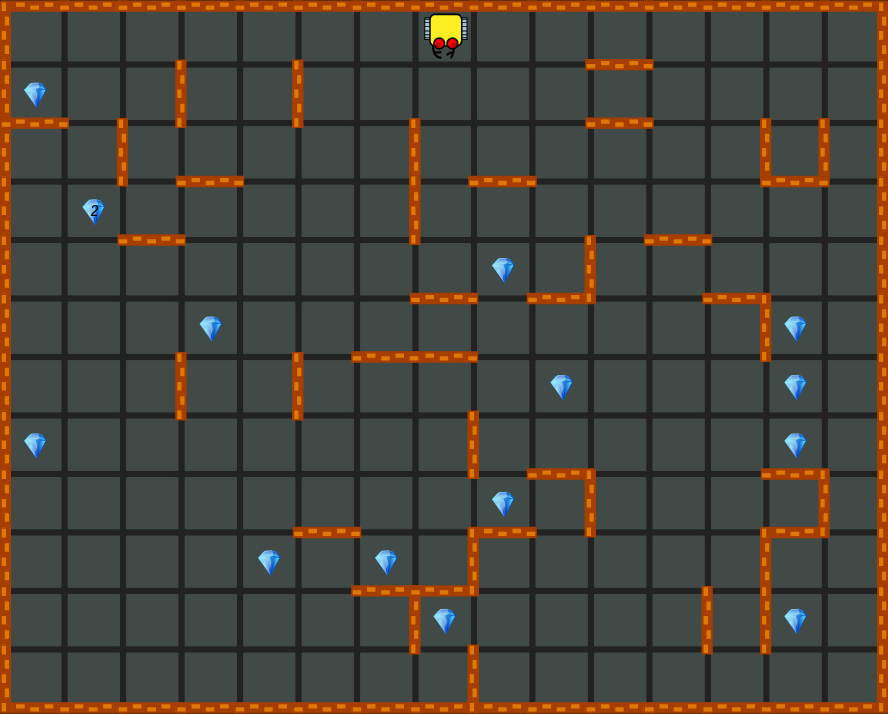
\includegraphics[height=0.4\textwidth]{imgk/variables2.png}
\end{center}
\vspace{-4mm}
\caption{Karel is reading his GPS device.}
\label{fig:var2s}
%\vspace{-1cm}
\end{figure}
\noindent
  \begin{itemize}
    \item A4: {\tt gpsx} is 7 and {\tt gpsy} is 11.
  \end{itemize}
\item What values will the variables {\tt gpsx} and {\tt gpsy} have after
Karel executes the following program? He starts from the position shown 
in Fig. \ref{fig:var2s}.
\begin{verbatim}
repeat 5
    while not wall
        go
        if gem
            get
    left
\end{verbatim}
  \begin{itemize}
    \item A2: {\tt gpsx} is 0 and {\tt gpsy} is 10.
  \end{itemize}
\item Which of the following programs is/are invalid?
  \begin{itemize}
    \item A3:
\begin{verbatim}
gpsx = 0
inc(gpsx)
\end{verbatim}
  \end{itemize}
\item Which of the following programs are invalid?
  \begin{itemize}
    \item A4:
\begin{verbatim}
proc count_steps
    while not wall
        go
        inc(n)
    return n
\end{verbatim}
  \end{itemize}
\end{enumerate}


\subsection{Programming exercises}

\subsubsection{H01 - Accounting}

\begin{verbatim}
def accounting
  num = zero
  while not empty
    put
    inc(num)
  return num

n = accounting
print "I have", n, "gems in the bag."
\end{verbatim}


\subsubsection{H02 - Tape Measure}

\begin{verbatim}
def measure
  # Go to the west wall
  # and turn east:
  while not north
    left
  left
  while not wall
    go
  repeat 2
    left
  # Start measuring:
  len = zero
  while not wall
    inc(len)
    go
  return len
  
l = measure
print "Width of the room is", l
\end{verbatim}


\subsubsection{H03 - Apple Orchard}

\begin{verbatim}
def orchard
  num = zero
  repeat 6
    # Check the tile you stand on:
    while gem
      inc(num)
    # Check the rest of the row:
    while not wall
      go
      while gem
        inc(num)
    # Move to next row and turn back:
    left
    if not wall
      go
    left
    # Check the tile you stand on:
    while gem
      inc(num)
    # Check the rest of the row:
    while not wall
      go
      while gem
        inc(num)
    # Move to next row and turn back:
    right
    if not wall
      go
    right

n = orchard
print "There are", n, "apples in the orchard."
\end{verbatim}


\subsubsection{H04 - New Carpet}

\begin{verbatim}
# Count tiles in one row. Assumes
# that Karel stands at the West end 
# of the row, facing East: 
def check_row
  n = 1
  while not wall
    go 
    inc(n)
  return n
  
# Assumes that Karel is at the 
# East end of a row, facing East:
def one_row_up
  finished = False
  left
  while wall
    left
    if not wall 
      go
    else 
      finished = True 
    right
  go
  return finished

# Move to the West end of row 
# and turn East. Assumes that 
# Karel faces North:
def get_west
  left
  while not wall
    go
  repeat 2
    left
  
# Measure the area:
def carpet
  a = check_row
  while one_row_up
    get_west
    inc(a, check_row)
  return a
  
# Calculate and print apartment area:
area = carpet
print "Carpet size =", area
\end{verbatim}


\section{Section I - Logic}

\subsection{Review questions}

\begin{enumerate}
\item Let's introduce a variable {\tt my\_age} that stores your age in years.
      This variable is:
  \begin{itemize}
    \item A1: Numerical.
  \end{itemize}
\item What is a {\em logical expression}? 
  \begin{itemize}
    \item A3: Expression that is either true or false.
  \end{itemize}
\item A is {\tt True} and B is {\tt False}. What is then the value of (A {\em and} {\em not} (A {\em or} B)) ?
  \begin{itemize}
    \item A1: {\tt False}.
  \end{itemize}
\item A is {\tt True} and B is {\tt True}. What is then the value of (A {\em and} {\em not} (A {\em and} {\em not} B)) ?
  \begin{itemize}
    \item A2: {\tt True}.
  \end{itemize}
\end{enumerate}

\subsection{Programming exercises}

\subsubsection{I01 - Reading Numbers}

\begin{verbatim}
# Make two steps:
def go2
  repeat 2 
    go

# Read number in box:
def readnumber
  # First detect gems
  # at key positions:
  go
  gem10 = gem
  go2
  gem12 = gem
  go2
  gem14 = gem
  right
  go
  right
  go
  gem23 = gem
  right
  go2
  gem03 = gem
  left
  go2
  gem01 = gem
  left
  go
  right
  go2
  repeat 2
    left
  
  # Decide what number is in 
  # the box:
  if gem10
    # 0, 2, 4, 5, 6, 8:
    if gem12
      # 2, 3, 5, 6, 8:
      if gem03
        # 5, 6, 8:
        if gem23
          # 4:
          return 4
        else
          # 5, 6:
          if gem01
            # 6:
            return 6
          else 
            # 5:
            return 5
    else
      # 0:
      return 0
  else
    # 1, 4, 7:
    if gem12
      # 4:
      return 4
    else
      # 1,7:
      if gem14
        # 7:
        return 7
      else
        # 1:
        return 1

# Main program:
n1 = readnumber
print "Number in the first box is", n1

# Move to second box:
right
repeat 3
  go
left

n2 = readnumber
print "Number in the second box is", n2

# Move to third box:
right
repeat 3
  go
left

n3 = readnumber
print "Number in the third box is", n3
\end{verbatim}

\subsubsection{I02 - Writing Numbers}

\begin{verbatim}
# Count gems.
def countgems
  num = 0
  while gem
    get
    inc(num)
  return num

def writenumber
  n = countgems
  print "Writing number", n
  go
  # Position [1, 0]:
  if n != 1 and n != 4 and n != 7
    put
  right
  go
  left
  # Position [2, 0]:
  put
  go
  # Position [2, 1]:
  if n != 2:
    put
  go
  # Position [2, 2]:
  put
  go
  # Position [2, 3]:
  if n != 5
    put
  go
  # Position [2, 4]:
  put
  left
  go
  # Position [1, 4]:
  if n != 1 and n != 4
    put
  go
  left
  # Position [0, 4]:
  if n != 1
    put
  go
  # Position [0, 3]:
  if n != 1 and n != 2 and n != 3 and n != 7
    put
  go
  # Position [0, 2]:
  if n != 1 and n != 7
    put
  # Position [1, 2]:
  if n == 8 
    left 
    go
    put
    repeat 2
      right
    go
    left
  go
  # Position [0, 1]:
  if n == 0 or n == 2 or n == 6 or n == 8
    put
  go
  left
  # Position [0, 0]:
  if n != 1 and n != 4 and n != 7
    put
  # Exit:
  go
  right
  repeat 2
    go
  repeat 2
    left
  
# Main program:
writenumber

# Move to the second box:
right
repeat 3
  go
left
writenumber

# Move to the third box:
right
repeat 3
  go
left
writenumber
\end{verbatim}

\subsubsection{I03 - Adding Numbers}

\begin{verbatim}
# Coming soon.
\end{verbatim}

\subsubsection{I04 - Eight Queens}

\begin{verbatim}
# Coming soon.
\end{verbatim}

\subsubsection{I05 - BubbleSort}

\begin{verbatim}
# Coming soon.
\end{verbatim}

%%%%%%%%%%%%%%%%%%%%%%%%%%%%%%%%%%%%%%%%%%%%%%%%%%%%%%%%%%%%%%%%%%%%%%%%%%%%%%%%%%%%%%%%

\part{Python}

\setcounter{section}{0}
\section{Introduction}

\subsection{Review questions}

\begin{enumerate}
\item What is the difference between a compiled and a scripting programming language?
  \begin{itemize}
    \item A4: Scripting languages do not require a compiler.
  \end{itemize}
\item What languages take better advantage of the underlying hardware architecture
      and why?
  \begin{itemize}
    \item A2: Compiled languages because the executable files are tailored 
          to the concrete hardware.
  \end{itemize}
\item Give three examples of compiled programming languages.
  \begin{itemize}
    \item A3: C, C++ and Fortran.
  \end{itemize}
\item Give three examples of interpreted programming languages.
  \begin{itemize}
    \item A3: Perl, Python and Ruby. 
  \end{itemize}
\item Where does the name "Python" of the programming language come from?
  \begin{itemize}
    \item A2: TV show in Great Britain.
  \end{itemize}
\item When was the implementation of Python started?
  \begin{itemize}
    \item A1: 1989
  \end{itemize}
\item Name three programming styles that Python permits.
  \begin{itemize}
    \item A2: Structured, object-oriented, functional.
  \end{itemize}
\item Name three programming styles that Python permits.
  \begin{itemize}
    \item A2: Structured, object-oriented, functional.
  \end{itemize}
\item How can displayed Python projects be cloned?
  \begin{itemize}
    \item A2: Through File Manager's {\em Project} menu.
  \end{itemize}
\item How can new Python project be launched?
  \begin{itemize}
    \item A2: Through the {\em Programming} menu.
    \item A3: Through File Manager's {\em Project} menu.
  \end{itemize}
\item How are Python programs processed in NCLab?
  \begin{itemize}
    \item A2: They are interpreted on a remote server.
  \end{itemize}
\item  What are the types of cells that a Python worksheet can contain?
  \begin{itemize}
    \item A2: Output cells.
    \item Input cells.
    \item Descriptive text cells.
  \end{itemize}
\item How can all input cells in a Python worksheet be evaluated at once?
  \begin{itemize}
    \item A4: By clicking on the blue arrow button in the menu.
  \end{itemize}
\item How can a single input cell be evaluated?
  \begin{itemize}
    \item A3: By clicking on {\tt run} under the input cell.
  \end{itemize}
\item What is the way to add a new input cell?
  \begin{itemize}
    \item A1: Click on {\tt add} under an input cell. 
    \item A4: Click on {\em New input cell} in {\em Edit} menu.
  \end{itemize}
\item How can a new text cell be added?
  \begin{itemize}
    \item A2: Click on {\em New text cell} in the {\em Edit} menu.
  \end{itemize}
\item What is the way to remove an input cell or a text cell?
  \begin{itemize}
    \item A1: Click on {\tt remove} under the cell. 
  \end{itemize}
\item How can an input cell be evaluated without using the mouse?
  \begin{itemize}
    \item A1: Hold CTRL and press ENTER.
    \item A2: Hold SHIFT and press ENTER.
  \end{itemize}
\item Which of the following are scientific libraries for Python?
  \begin{itemize}
    \item A2: Numpy.
    \item A3: Scipy.
    \item A4: Sympy.
  \end{itemize}
\end{enumerate}

\subsection{Programming exercises}

Coming soon.


\section{Using Python as Graphing Calculator}

\subsection{Review questions}

\begin{enumerate}
\item What is the result of $11 / 4$ in Python?
  \begin{itemize}
    \item A2: {\tt 2}
  \end{itemize}
\item Type $3^2$ using Python syntax:
  \begin{itemize}
    \item A4: {\tt 3**2}
  \end{itemize}
\item Type $5$ modulo $2$ using Python syntax:
  \begin{itemize}
    \item A2: {\tt 5 \% 2}
  \end{itemize}
\item What is the result of $1**4*2$ in Python?
  \begin{itemize}
    \item A3: {\tt 2}
  \end{itemize}
\item What do we need to type into an empty Python worksheet in order to evaluate sin($\pi/4$)?
  \begin{itemize}
    \item A2:
\begin{verbatim}
from numpy import sin, pi
sin(pi/4)
\end{verbatim}
  \end{itemize}
\item Which of the following are correct ways to define a complex number?
  \begin{itemize}
    \item A1: {\tt 2 + 3j}
    \item A2: {\tt 2 + 3J}
  \end{itemize}
\item Which of the following codes will draw a square with vertices [0, 0], [1, 0], [1, 1], [0, 1]?
  \begin{itemize}
    \item A3:
\begin{verbatim}
from pylab import *
x = [0.0, 1.0, 1.0, 0.0, 0.0]
y = [0.0, 0.0, 1.0, 1.0, 0.0]
clf()
plot(x, y)
lab.show()
\end{verbatim}
  \end{itemize}
\item Which of the following codes will plot a cosine function in the interval $(0, \pi)$ using dashed green line with
the step 0.01?
  \begin{itemize}
    \item A2:
\begin{verbatim}
from numpy import cos, pi
from pylab import *
x = arange(0, pi, 0.01)
y = cos(x)
clf()
plot(x, y, 'g--')
lab.show()
\end{verbatim}
  \end{itemize}
\end{enumerate}

\subsection{Programming exercises}

Coming soon.


\section{More on Functions}

\subsection{Review questions}

\begin{enumerate}
\item Why do we define {\em functions} in programming? 
  \begin{itemize}
    \item A1: To isolate self-contained functionality and make it easily reusable.
  \end{itemize}
\item Which of the following are correct function definitions?
  \begin{itemize}
    \item A2:
\begin{verbatim}
def subtract(a, b):
    return a - b
\end{verbatim}
    \item A4:
\begin{verbatim}
def subtract(a, b = 5):
    return a - b
\end{verbatim}
  \end{itemize}
\item When do we have to specify argument types in Python functions?
  \begin{itemize}
    \item A1: Never
  \end{itemize}
\item The modulo operation calculates the 
      rest after integer division. Assume positive integers $a > 0$ and $b > 0$.
      The number $a$ can be decomposed as follows:
      $$
      a = nb + r
      $$  
      where $n \ge 0$ and $0 \le r < b$ are integers.
      Which of the following functions will do the job
      and return the numbers {\tt nb} and {\tt r} ?
  \begin{itemize}
    \item A2:
\begin{verbatim}
def splitnumber(a, b):
    return a - a % b, a % b
\end{verbatim}
  \end{itemize}
\item Of the following four functions, choose the best one to calculate the hypotenuse
      of a right-angled triangle when you know that most of the time one of its shorter
      edges will be 5 cm long.
  \begin{itemize}
    \item A3:
\begin{verbatim}
from numpy import sqrt
def hypotenuse(a, b = 5):
    return sqrt(a**2 + b**2)
\end{verbatim}
  \end{itemize}
\end{enumerate}


\subsection{Programming exercises}

Coming soon.


\section{More on Variables}

\subsection{Review questions}

\begin{enumerate}
\item Which of the following Python programs are invalid?
  \begin{itemize}
    \item A2
    \item A3
    \item A4
  \end{itemize}
\item When can a given variable have different types in a Python program?
  \begin{itemize}
    \item A1: Any time.
  \end{itemize}
\item We have two variables {\tt a} and {\tt b} and need to swap their values. Which of the 
following codes will do it?
  \begin{itemize}
    \item A4:
\begin{verbatim}
c = a
a = b
b = c
\end{verbatim}
  \end{itemize}
\item Should we preferably use local variables, or global variables, and why?
  \begin{itemize}
    \item A4: Local variables because our code is less prone to mistakes. 
  \end{itemize}
\item Should we use global variables in functions and why?
  \begin{itemize}
    \item A3: No, it makes the code less transparent and more prone to mistakes.
  \end{itemize}
\item What is shadowing of variables?
  \begin{itemize}
    \item A4: There is a local variable whose name matches the name of a global one.
  \end{itemize}
\end{enumerate}


\subsection{Programming exercises}

Coming soon.


\section{Review of Logic}

\subsection{Review questions}

\begin{enumerate}
\item Let {\tt a} and {\tt b} be Boolean variables. What is the 
result of {\tt (a or b) or (not (a or b))}
  \begin{itemize}
    \item A4: True
  \end{itemize}
\item Let {\tt a} and {\tt b} be Boolean variables. What is the 
result of {\tt (a and b) and (not (a and b))}
  \begin{itemize}
    \item A4: False
  \end{itemize}
\end{enumerate}

\subsection{Programming exercises}

Coming soon.


\section{More on Conditions and the {\tt while} Loop}

\subsection{Review questions}

\begin{enumerate}
\item When should the {\tt elif} statement be used?
  \begin{itemize}
    \item A2: When there are more than two options in the {\tt if - else} condition. 
  \end{itemize}
\item When should the {\tt while} loop be used?
  \begin{itemize}
    \item A4: When the number of repetitions is not know a priori.
  \end{itemize}
\item What is the purpose of the {\tt break} statement?
  \begin{itemize}
    \item A4: Exit a loop. If multiple loops are embedded, exit just the closest one.
  \end{itemize}
\item What will the output of the following program be?
\begin{verbatim}
a = 0
while True:
    a += 1
    if a < 8:
        continue
    print a
    break
\end{verbatim}
  \begin{itemize}
    \item A4:
\begin{verbatim}
8
\end{verbatim}
  \end{itemize}
\item What is the Newton's method?
  \begin{itemize}
    \item A2: Method to approximate solutions to nonlinear equations.
  \end{itemize}
\end{enumerate}


\subsection{Programming exercises}

Coming soon.

\section{Strings}

\subsection{Review questions}

\begin{enumerate}
\item What of the following are correct ways to include quotes in a string?
  \begin{itemize}
    \item A3:
\begin{verbatim}
"I say \"goodbye\", you say \"hello\""
\end{verbatim}
    \item A4:
\begin{verbatim}
"I say \'goodbye\', you say \'hello\'"
\end{verbatim}
  \end{itemize}
\item What of the following are correct ways to define a multiline string?
  \begin{itemize}
    \item A2:
\begin{verbatim}
"""\
I say "High", you say "Low".
You say "Why?" And I say "I don't know".\
"""
\end{verbatim}
  \end{itemize}
\item What output will be produced by the following code?
\begin{verbatim}
s1 = "Thank you"
s2 = "very"
s3 = "much!"
print s1 + 5*s2 + s3
\end{verbatim}
  \begin{itemize}
    \item A2:
\begin{verbatim}
Thank youveryveryveryveryverymuch!
\end{verbatim}
  \end{itemize}
\item What output will be produced by the following code?
\begin{verbatim}
s1 = "intermediate"
s2 = s1[7] + s1[4] + s1[3] + s1[6] + s1[5]
print s2
\end{verbatim}
  \begin{itemize}
    \item A2:
\begin{verbatim}
dreem
\end{verbatim}
  \end{itemize}
\item What output will be produced by the following code?
\begin{verbatim}
s1 = "intermediate"
s2 = s1[:5]
print s2
s3 = s1[5:10]
print s3
s4 = s1[-2] + s1[-1]
print s4
\end{verbatim}
  \begin{itemize}
    \item A3:
\begin{verbatim}
inter
media
te
\end{verbatim}
  \end{itemize}
\item What is the correct way to measure and print the length of a string {\tt str}?
  \begin{itemize}
    \item A2:
\begin{verbatim}
print len(str)
\end{verbatim}
  \end{itemize}
\item What will the output of the following code be?
\begin{verbatim}
print range(2, 5)
\end{verbatim}
  \begin{itemize}
    \item A3:
\begin{verbatim}
[2, 3, 4]
\end{verbatim}
  \end{itemize}
\item What output corresponds to the following code?
\begin{verbatim}
word = "breakfast"
for m in range(5, 9):
    print word[m]
\end{verbatim}
  \begin{itemize}
    \item A3:
\begin{verbatim}
f
a
s
t
\end{verbatim}
  \end{itemize}
\end{enumerate}

\subsection{Programming exercises}

Coming soon.

\section{Tuples, Lists, and Dictionaries}

\subsection{Review questions}

\begin{enumerate}
\item What is the variable {\tt var}?
\begin{verbatim}
var = (1, 2, 3, 'A', 'B', 'C', "alpha", "beta", "gamma")
\end{verbatim}
  \begin{itemize}
    \item A2: Tuple.
  \end{itemize}
\item What will the output of the following program be?
  \begin{itemize}
    \item A2:
\begin{verbatim}
C
(1, 2, 3)
('alpha', 'beta')
\end{verbatim}
  \end{itemize}
\item Can new items be added to a tuple?
  \begin{itemize}
    \item A3: No.
  \end{itemize}
\item What is the correct way to determine the length of a tuple {\tt T}?
  \begin{itemize}
    \item A3:
\begin{verbatim}
len(T)
\end{verbatim}
  \end{itemize}
\item What is the variable {\tt var}?
\begin{verbatim}
names = ["John", "Jake", "Josh"]
\end{verbatim}
  \begin{itemize}
    \item A1: List.
  \end{itemize}
\item Identify the output of the following code:
\begin{verbatim}
names = ["John", "Jake", "Josh"]
name = names.del[1]
print name
\end{verbatim}
  \begin{itemize}
    \item A4: Error message.
  \end{itemize}
\item Identify the output of the following code:
\begin{verbatim}
names = ["John", "Jake", "Josh"]
names.append("Jerry")
print names
\end{verbatim}
  \begin{itemize}
    \item A1:
\begin{verbatim}
['John', 'Jake', 'Josh', 'Jerry']
\end{verbatim}
  \end{itemize}
\item Identify the output of the following code:
\begin{verbatim}
names = ["John", "Jake", "Josh"]
names.pop(0)
print names
\end{verbatim}
  \begin{itemize}
    \item A1:
\begin{verbatim}
['Jake', 'Josh']
\end{verbatim}
  \end{itemize}
\item Identify the output of the following code:
\begin{verbatim}
names = ["John", "Jake", "Josh"]
names.insert(1, "Jenny")
print names
\end{verbatim}
  \begin{itemize}
    \item A2:
\begin{verbatim}
['John', 'Jenny', 'Jake', 'Josh']
\end{verbatim}
  \end{itemize}
\item Identify the output of the following code:
  \begin{itemize}
    \item A3:
\begin{verbatim}
['Josh', 'Jake', 'John']
\end{verbatim}
  \end{itemize}
\item Identify the output of the following code:
\begin{verbatim}
names = ["John", "Jerry", "Jake", "Josh", "Jerry"]
names.sort()
print names
\end{verbatim}
  \begin{itemize}
    \item A2:
\begin{verbatim}
['Jake', 'Jerry', 'Jerry', 'John', 'Josh']
\end{verbatim}
  \end{itemize}
\item Identify the output of the following code:
\begin{verbatim}
names = ["John", "Jerry", "Jake", "Josh", "Jerry"]
print names.count("Jerry")
\end{verbatim}
  \begin{itemize}
    \item A2: {\tt 2}
  \end{itemize}
\item Identify the output of the following code:
\begin{verbatim}
names = ["John", "Jerry", "Jake", "Josh", "Jerry"]
print names.index("Jerry")
\end{verbatim}
  \begin{itemize}
    \item A1: {\tt 1}
  \end{itemize}
\item Identify the output of the following code:
\begin{verbatim}
A = ["John", "Jerry", "Jed"]
B = ['1', '2', '3']
print zip(A, B)
\end{verbatim}
  \begin{itemize}
    \item A4:
\begin{verbatim}
[('John', '1'), ('Jerry', '2'), ('Jed', '3')]
\end{verbatim}
  \end{itemize}
\item What is the correct way to define a dictionary {\tt D} containing the 
      English words "city", "fire", "sun" and their Spanish translations "ciudad",
      "fuego", and "sol" ?
  \begin{itemize}
    \item A1:
\begin{verbatim}
D = {'city': 'ciudad', 'fire': 'fuego', 'sun': 'sol'}
\end{verbatim}
    \item A2:
\begin{verbatim}
D = {'fire': 'fuego', 'sun': 'sol', 'city': 'ciudad'}
\end{verbatim}
    \item A3:
\begin{verbatim}
D = {'sun': 'sol', 'fire': 'fuego', 'city': 'ciudad'}
\end{verbatim}
    \item A4:
\begin{verbatim}
D = {'fire': 'fuego', 'city': 'ciudad', 'sun': 'sol'}
\end{verbatim}
  \end{itemize}
\item What is the correct way to add to a dictionary {\tt D} new key 
"school" whose value is "escuela"? 
  \begin{itemize}
    \item A3:
\begin{verbatim}
D['school'] = 'escuela'
\end{verbatim}
  \end{itemize}
\item A dictionary {\tt D} is defined below. What is the correct way to print the value for 
the key "city"?
\begin{verbatim}
D = {'fire': 'fuego', 'city': 'ciudad', 'sun': 'sol'}
\end{verbatim}
  \begin{itemize}
    \item A2:
\begin{verbatim}
print D['city']
\end{verbatim}
  \end{itemize}
\item A dictionary {\tt D} is defined below. What is the correct way to ascertain whether
or not the key "sun" is present?
\begin{verbatim}
D = {'fire': 'fuego', 'city': 'ciudad', 'sun': 'sol'}
\end{verbatim}
  \begin{itemize}
    \item A4:
\begin{verbatim}
D.has_key('sun')
\end{verbatim}
  \end{itemize}
\item A dictionary {\tt D} is defined below. What is the correct way to print 
all keys?
\begin{verbatim}
D = {'fire': 'fuego', 'city': 'ciudad', 'sun': 'sol'}
\end{verbatim}
  \begin{itemize}
    \item A4:
\begin{verbatim}
print D.keys()
\end{verbatim}
  \end{itemize}
\item A dictionary {\tt D} is defined below. What is the correct way to print 
all values?
\begin{verbatim}
D = {'fire': 'fuego', 'city': 'ciudad', 'sun': 'sol'}
\end{verbatim}
  \begin{itemize}
    \item A4:
\begin{verbatim}
print D.values()
\end{verbatim}
  \end{itemize}
\end{enumerate}


\subsection{Programming exercises}

Coming soon.


\section{The {\tt for} Loop} 

\subsection{Review questions}

\begin{enumerate}
\item What language element in Karel the Robot is most similar to the {\tt for} loop in Python.
  \begin{itemize}
    \item A3: The {\tt repeat} command.
  \end{itemize}
\item When should the {\tt for} loop be used?
  \begin{itemize}
    \item A1: When we need to go through a list or tuple.
    \item A2: When the number of repetitions is known a priori. 
  \end{itemize}
\item Which of the following codes will print numbers 4, 5, 6, 7, 8, 9?
  \begin{itemize}
    \item A2:
\begin{verbatim}
L = range(4, 10)
for number in L:
    print number
\end{verbatim}
    \item A3:
\begin{verbatim}
for val in range(4:10):
    print val
\end{verbatim}
  \end{itemize}
\end{enumerate}

\subsection{Programming exercises}

Coming soon.


\section{Catching and Raising Exceptions}

\subsection{Review questions}

\begin{enumerate}
\item What do we mean by an {\em exception} in programming?
  \begin{itemize}
    \item A2: Exceptional situation in the code leading to an error. 
  \end{itemize}
\item Identify valid exceptions in Python.
  \begin{itemize}
    \item A1: {\tt IndentationError}
    \item A2: {\tt UnboundLocalError}
    \item A4: {\tt OverflowError}
  \end{itemize}
\item What does {\tt assert(x != 0)} do if {\tt x} is zero?
  \begin{itemize}
    \item A3: Raises the {\tt AssertionError} exception.
  \end{itemize}
\item What is the correct way to raise a {\tt ValueError} exception 
      when {\tt x} is greater than five?
  \begin{itemize}
    \item A2:
\begin{verbatim}
if x > 5:
    raise ValueError("x should be <= five!")
\end{verbatim}
  \end{itemize}
\end{enumerate}


\subsection{Programming exercises}

Coming soon.

\section{Object-Oriented Programming}

\subsection{Review questions}

\begin{enumerate}
\item The philosophy of object-oriented programming is:
  \begin{itemize}
    \item A3: Use entities that combine functionality and data.
  \end{itemize}
\item What is the relation between {\em class} and {\em object} in object-oriented programming?
  \begin{itemize}
    \item A4: Object is an instance (concrete realization) of a class.
  \end{itemize}
\item What are {\em methods} of a class?
  \begin{itemize}
    \item A4: Functions that are part of the class definition.
  \end{itemize}
\item Where are methods defined and where are they used?
  \begin{itemize}
    \item A3: They are defined in a class and used by instances of the class.
  \end{itemize}
\item Can methods of a class operate with data not owned by the class and when?
  \begin{itemize}
    \item A1: Yes, always.
  \end{itemize}
\item What is a {\em constructor}?
  \begin{itemize}
    \item A1: Method of a class that is used to initialize newly created instances.
  \end{itemize}
\item What is the correct way to define a constructor that initializes a variable
      {\tt A} in a class with a value {\tt a}?
  \begin{itemize}
    \item A3:
\begin{verbatim}
    def __init__(self, a):
        self.A = a
\end{verbatim}
  \end{itemize}
\item A class contains a variable {\tt A}. What is the correct way to define 
      a method {\tt printdata} of this class that prints the value of the variable?
  \begin{itemize}
    \item A4:
\begin{verbatim}
    def printdata(self):
        print "A =", self.A
\end{verbatim}
  \end{itemize}
\item Given a text string {\tt S}, what is the correct way to count and print the number 
      of appearances of another string {\tt word} in {\tt S}?
  \begin{itemize}
    \item A3:
\begin{verbatim}
    print S.count(word)
\end{verbatim}
    \end{itemize}
\item What is the way to check whether a string {\tt S} is a number?
  \begin{itemize}
    \item A1:
\begin{verbatim}
    S.isdigit()
\end{verbatim}
    \end{itemize}
\item What is the way to replace in a text string {\tt S} a string {\tt s1} with another string {\tt s2}?
  \begin{itemize}
    \item A4:
\begin{verbatim}
    S.replace(s1, s2)
\end{verbatim}
    \end{itemize}
\item How can be in Python a string {\tt S} converted to uppercase?
  \begin{itemize}
    \item A3:
\begin{verbatim}
    S.upper()
\end{verbatim}
  \end{itemize}

\end{enumerate}


\subsection{Programming exercises}

Coming soon.

\section{Class Inheritance}

\subsection{Review questions}

\begin{enumerate}
\item When should inheritance be used in object-oriented programming?
  \begin{itemize}
    \item A2: When some functionality is common to multiple classes.
  \end{itemize}
\item What is the correct way to define a new class {\tt B} which is a descendant of 
      class {\tt A}?
  \begin{itemize}
    \item A1:
\begin{verbatim}
class B(A):
\end{verbatim}
  \end{itemize}
\item What is the correct way to call from a descendant class {\tt B} the constructor of its parent class 
      {\tt A}?
  \begin{itemize}
    \item A1:
\begin{verbatim}
def __init__(self):
    A.__init__(self)
\end{verbatim}
  \end{itemize}
\end{enumerate}



\subsection{Programming exercises}

Coming soon.



\end{document}

 
